

% Gradient Info
  
\tikzset {_mzix41zd3/.code = {\pgfsetadditionalshadetransform{ \pgftransformshift{\pgfpoint{0 bp } { 0 bp }  }  \pgftransformrotate{-270 }  \pgftransformscale{2 }  }}}
\pgfdeclarehorizontalshading{_buy4zbb99}{150bp}{rgb(0bp)=(1,1,1);
rgb(54.82142857142857bp)=(1,1,1);
rgb(62.5bp)=(0.61,0.61,0.61);
rgb(100bp)=(0.61,0.61,0.61)}

% Gradient Info
  
\tikzset {_mg3p0nsm3/.code = {\pgfsetadditionalshadetransform{ \pgftransformshift{\pgfpoint{0 bp } { -0.5 bp }  }  \pgftransformrotate{-90 }  \pgftransformscale{2 }  }}}
\pgfdeclarehorizontalshading{_je6tgefoc}{150bp}{rgb(0bp)=(1,1,1);
rgb(37.5bp)=(1,1,1);
rgb(62.5bp)=(0,0,0);
rgb(100bp)=(0,0,0)}
\tikzset{_rhzzu6zch/.code = {\pgfsetadditionalshadetransform{\pgftransformshift{\pgfpoint{0 bp } { -0.5 bp }  }  \pgftransformrotate{-90 }  \pgftransformscale{2 } }}}
\pgfdeclarehorizontalshading{_y9hn7kdjv} {150bp} {color(0bp)=(transparent!0);
color(37.5bp)=(transparent!0);
color(62.5bp)=(transparent!10);
color(100bp)=(transparent!10) } 
\pgfdeclarefading{_vng0zxtvy}{\tikz \fill[shading=_y9hn7kdjv,_rhzzu6zch] (0,0) rectangle (50bp,50bp); } 

% Gradient Info
  
\tikzset {_bj5c9j7rb/.code = {\pgfsetadditionalshadetransform{ \pgftransformshift{\pgfpoint{0 bp } { 0 bp }  }  \pgftransformrotate{-90 }  \pgftransformscale{2 }  }}}
\pgfdeclarehorizontalshading{_qk2kexk1u}{150bp}{rgb(0bp)=(1,0,0);
rgb(49.64285714285714bp)=(1,0,0);
rgb(50.714285714285715bp)=(1,0,0);
rgb(57.23214285714286bp)=(0.29,0.56,0.89);
rgb(100bp)=(0.29,0.56,0.89)}

% Gradient Info
  
\tikzset {_r32u86fl6/.code = {\pgfsetadditionalshadetransform{ \pgftransformshift{\pgfpoint{0 bp } { 0 bp }  }  \pgftransformrotate{-270 }  \pgftransformscale{2 }  }}}
\pgfdeclarehorizontalshading{_hhq9tjtq2}{150bp}{rgb(0bp)=(1,1,1);
rgb(54.82142857142857bp)=(1,1,1);
rgb(62.5bp)=(0.61,0.61,0.61);
rgb(100bp)=(0.61,0.61,0.61)}

% Gradient Info
  
\tikzset {_nkdpehyiu/.code = {\pgfsetadditionalshadetransform{ \pgftransformshift{\pgfpoint{0 bp } { -0.5 bp }  }  \pgftransformrotate{-90 }  \pgftransformscale{2 }  }}}
\pgfdeclarehorizontalshading{_pyxk87nd7}{150bp}{rgb(0bp)=(1,1,1);
rgb(37.5bp)=(1,1,1);
rgb(62.5bp)=(0,0,0);
rgb(100bp)=(0,0,0)}
\tikzset{_mwfa1wyeu/.code = {\pgfsetadditionalshadetransform{\pgftransformshift{\pgfpoint{0 bp } { -0.5 bp }  }  \pgftransformrotate{-90 }  \pgftransformscale{2 } }}}
\pgfdeclarehorizontalshading{_jy97qok0z} {150bp} {color(0bp)=(transparent!0);
color(37.5bp)=(transparent!0);
color(62.5bp)=(transparent!10);
color(100bp)=(transparent!10) } 
\pgfdeclarefading{_wpyz07rb3}{\tikz \fill[shading=_jy97qok0z,_mwfa1wyeu] (0,0) rectangle (50bp,50bp); } 

% Gradient Info
  
\tikzset {_lc7ue9dpu/.code = {\pgfsetadditionalshadetransform{ \pgftransformshift{\pgfpoint{0 bp } { 0 bp }  }  \pgftransformrotate{-90 }  \pgftransformscale{2 }  }}}
\pgfdeclarehorizontalshading{_ayppihpkw}{150bp}{rgb(0bp)=(1,0,0);
rgb(37.5bp)=(1,0,0);
rgb(49.19642857142857bp)=(1,0,0);
rgb(58.125bp)=(0.29,0.56,0.89);
rgb(62.5bp)=(0.29,0.56,0.89);
rgb(100bp)=(0.29,0.56,0.89)}
\tikzset{every picture/.style={line width=0.75pt}} %set default line width to 0.75pt        

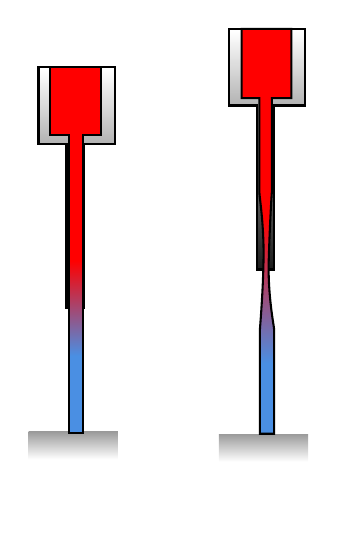
\begin{tikzpicture}[x=0.75pt,y=0.75pt,yscale=-1,xscale=1]
%uncomment if require: \path (0,300); %set diagram left start at 0, and has height of 300

%Shape: Square [id:dp10477043116887463] 
\draw  [draw opacity=0][shading=_buy4zbb99,_mzix41zd3] (115,209.33) -- (158,209.33) -- (158,252.33) -- (115,252.33) -- cycle ;
%Shape: Path Data [id:dp6696875766682748] 
\path  [shading=_je6tgefoc,_mg3p0nsm3,path fading= _vng0zxtvy ,fading transform={xshift=2}] (141.7,149.55) -- (133.2,149.55) -- (133.2,70.55) -- (119.7,70.55) -- (119.7,33.55) -- (156.7,33.55) -- (156.7,70.55) -- (141.7,70.55) -- (141.7,149.55) -- cycle ; % for fading 
 \draw   (141.7,149.55) -- (133.2,149.55) -- (133.2,70.55) -- (119.7,70.55) -- (119.7,33.55) -- (156.7,33.55) -- (156.7,70.55) -- (141.7,70.55) -- (141.7,149.55) -- cycle ; % for border 

%Shape: Path Data [id:dp6744062824884621] 
\path  [shading=_qk2kexk1u,_bj5c9j7rb] (141,209.8) -- (134.2,209.8) -- (134.2,66.4) -- (125.4,66.4) -- (125.4,33.8) -- (150,33.8) -- (150,66.4) -- (141,66.4) -- (141,209.8) -- cycle ; % for fading 
 \draw   (141,209.8) -- (134.2,209.8) -- (134.2,66.4) -- (125.4,66.4) -- (125.4,33.8) -- (150,33.8) -- (150,66.4) -- (141,66.4) -- (141,209.8) -- cycle ; % for border 

%Shape: Square [id:dp5760880909889591] 
\draw  [draw opacity=0][shading=_hhq9tjtq2,_r32u86fl6] (206.6,210.53) -- (249.6,210.53) -- (249.6,253.53) -- (206.6,253.53) -- cycle ;
%Shape: Path Data [id:dp31004184155496395] 
\path  [shading=_pyxk87nd7,_nkdpehyiu,path fading= _wpyz07rb3 ,fading transform={xshift=2}] (233.3,131.15) -- (224.8,131.15) -- (224.8,52.15) -- (211.3,52.15) -- (211.3,15.15) -- (248.3,15.15) -- (248.3,52.15) -- (233.3,52.15) -- (233.3,131.15) -- cycle ; % for fading 
 \draw   (233.3,131.15) -- (224.8,131.15) -- (224.8,52.15) -- (211.3,52.15) -- (211.3,15.15) -- (248.3,15.15) -- (248.3,52.15) -- (233.3,52.15) -- (233.3,131.15) -- cycle ; % for border 

%Shape: Path Data [id:dp09202608753864516] 
\path  [shading=_ayppihpkw,_lc7ue9dpu] (233.22,210.31) -- (226.4,210.31) -- (226.4,159.93) .. controls (226.4,159.91) and (226.4,159.9) .. (226.4,159.89) .. controls (226.47,158.49) and (227.89,142.35) .. (228.14,125.98) .. controls (228.39,109.6) and (226.17,96.25) .. (226.14,94.15) -- (226.14,94.15) -- (226.14,94.15) .. controls (226.14,94.14) and (226.14,94.13) .. (226.14,94.12) -- (226.14,48.56) -- (217.59,48.56) -- (217.59,15.22) -- (241.59,15.22) -- (241.59,48.56) -- (232.12,48.56) -- (232.12,94) .. controls (232.12,94.05) and (232.12,94.1) .. (232.12,94.15) .. controls (231.96,96.1) and (231.14,109.6) .. (230.64,126.73) .. controls (230.14,143.85) and (233.22,158.6) .. (233.22,159.89) -- (233.22,210.31) -- cycle ; % for fading 
 \draw   (233.22,210.31) -- (226.4,210.31) -- (226.4,159.93) .. controls (226.4,159.91) and (226.4,159.9) .. (226.4,159.89) .. controls (226.47,158.49) and (227.89,142.35) .. (228.14,125.98) .. controls (228.39,109.6) and (226.17,96.25) .. (226.14,94.15) -- (226.14,94.15) -- (226.14,94.15) .. controls (226.14,94.14) and (226.14,94.13) .. (226.14,94.12) -- (226.14,48.56) -- (217.59,48.56) -- (217.59,15.22) -- (241.59,15.22) -- (241.59,48.56) -- (232.12,48.56) -- (232.12,94) .. controls (232.12,94.05) and (232.12,94.1) .. (232.12,94.15) .. controls (231.96,96.1) and (231.14,109.6) .. (230.64,126.73) .. controls (230.14,143.85) and (233.22,158.6) .. (233.22,159.89) -- (233.22,210.31) -- cycle ; % for border 





\end{tikzpicture}
